\clearpage

\section{QuantumChannelDv}

\begin{tcolorbox}	
\begin{tabular}{p{2.75cm} p{0.2cm} p{10.5cm}} 	
\textbf{Header File}   &:& quantum\_channel\_dv.h \\
\textbf{Source File}   &:& quantum\_channel\_dv.cpp \\
\textbf{Version}       &:& 20190410
\end{tabular}
\end{tcolorbox}

\maketitle
This block emulates a quantum channel using discrete variables. In this way, a single-photon inputs the block and suffers the attenuation and birefringence effects inherent to a real optical fiber channel. QuantumChannelDv block accepts the following input signal,

\begin{itemize}
  \item inputSignal[0] $\rightarrow$ AliceQTx\_Out (PhotonStreamXY).

\end{itemize}
It produces PhotonStreamXY signal which comprises the encoded single photons after suffering optical fiber channel effects,
\begin{itemize}
  \item outputSignal[0] $\rightarrow$ BobQRx\_In (PhotonStreamXY)
\end{itemize}

It also accepts four input parameters listed below.

\subsection*{Input Parameters}

	\begin{itemize}
        \item double attenuationDbm\_perKm - It is the attenuation in dB per km. Its default value is 0.0.

        \item double fiberLength - It is the length of the channel optical fiber in km. Its default value is 1.0.

		\item sop\_rotation\_type channelType - This value selects the channelType which can take the values \textit{Determinist} or \textit{Stocastic}. Its default value is \textit{Stocastic}.
	
		\item double polLineWidth - This value depends on the velocity that we want polarization changes with time. It is only used in \textit{Stocastic} channel type. Its default value is $900\times10^{-9}$ Hz.

	\end{itemize}

\subsection*{Methods}
\begin{itemize}
        \item void setAtennuationDbmPerKm(double att) - This method allows to set the attenuation in Db per km.

        \item void setFiberLength(double fLength) - This method allows to set the length of the optical fiber channel.

		\item void setFiberModel(sop\_rotation\_type fModel) - This method allows to set the channel type.
	
		\item void setPolarizationLinewidth(double pLinewidth) - This method allows to set the polarization linewidth in Hz.
	\end{itemize}

\subsection*{Functional description}

\begin{figure}[h]
	\centering
	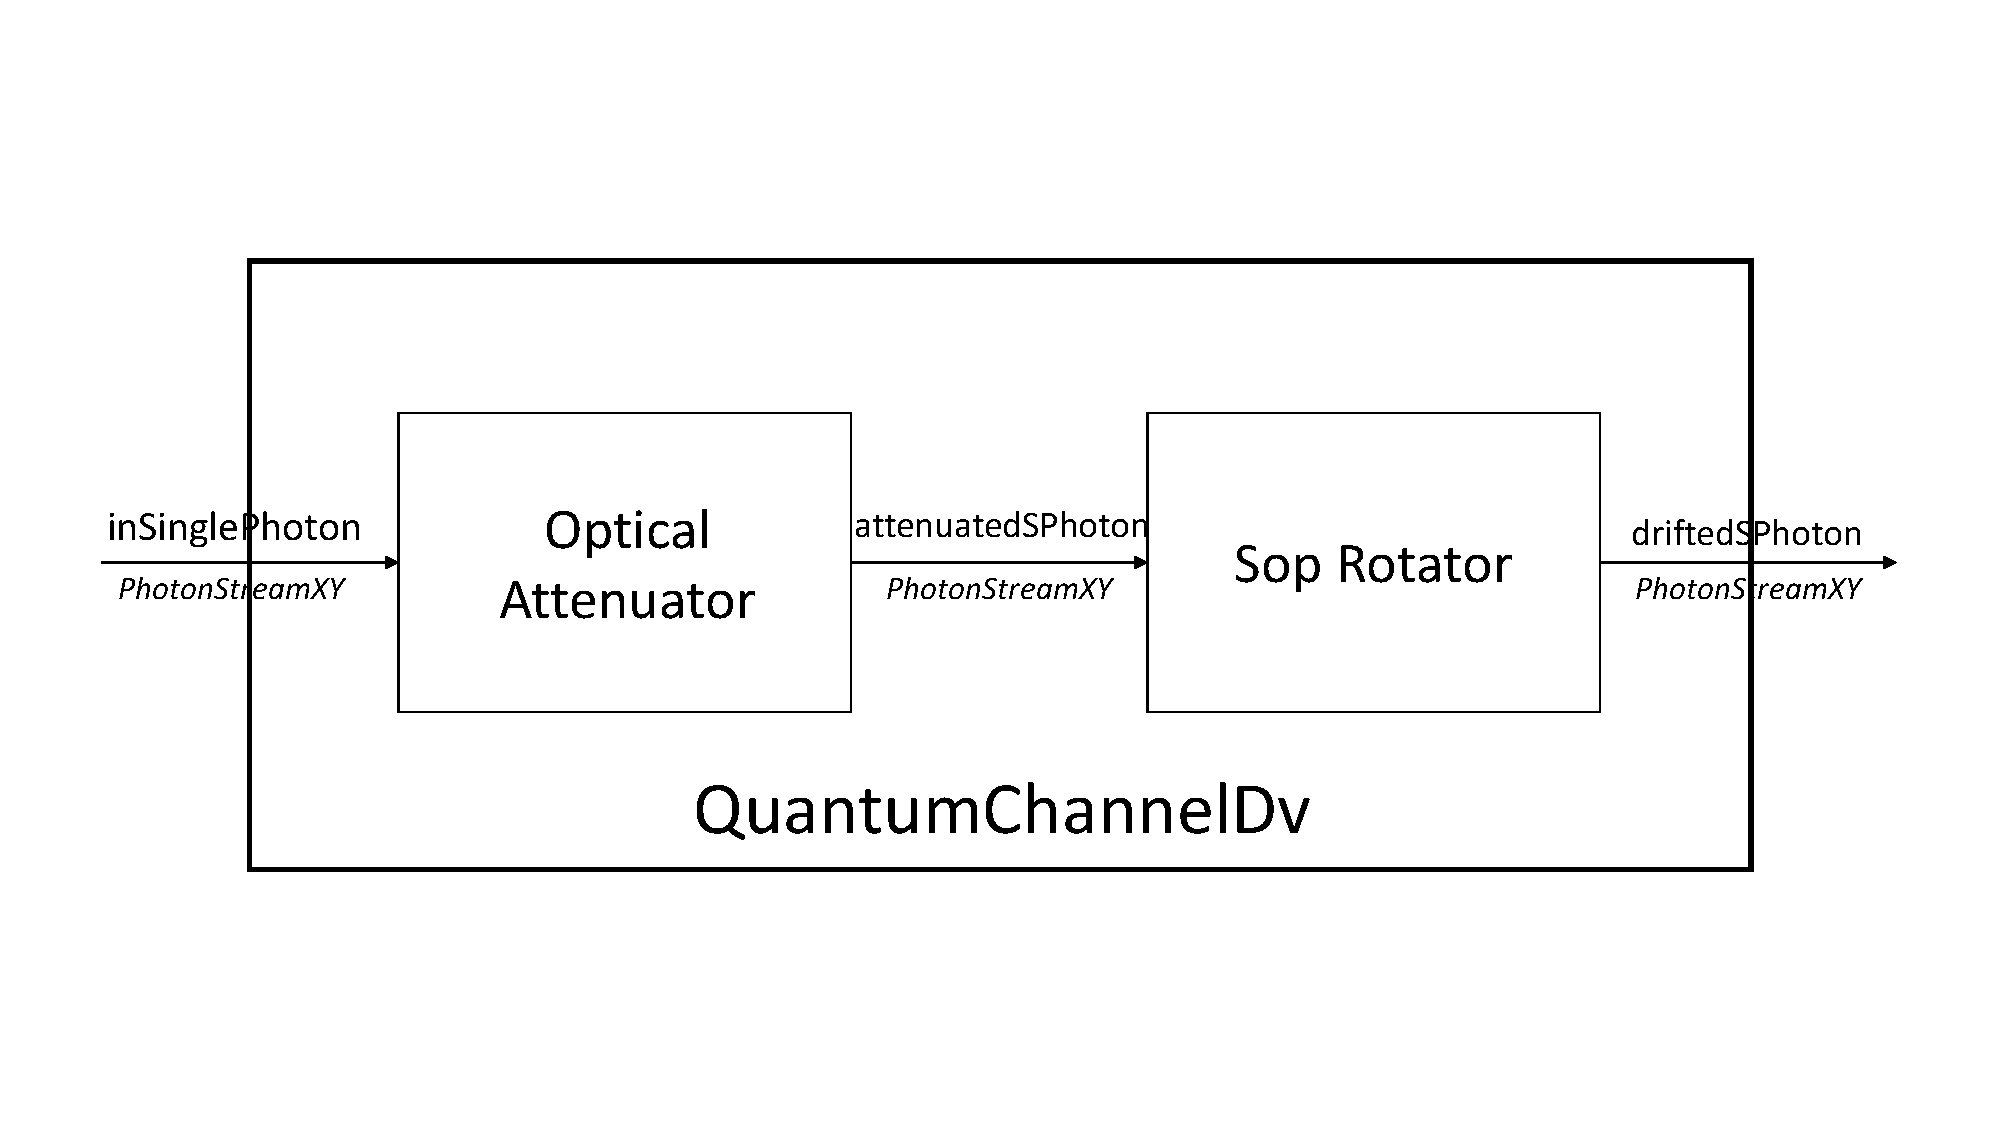
\includegraphics[clip, trim=0.5cm 2.0cm 0.5cm 2cm, width=1.0\textwidth]{./lib/QuantumChannelDv/figures/QuantumChannelDv_diagram.pdf}
	\caption{Schematic of Quantum Channel using discrete variables}\label{QuantumChannelDvDiagram}
\end{figure}

This block receives 1 input PhotonStreamXY signal, and outputs also a PhotonStreamXY signal. It attenuates the signal according with the input parameters introduced through the block optical attenuator (a more detailed description about this block can be found in \textsc{lib/optical\_attenuator}). The attenuated single-photon outputs the optical attenuator block and inputs a SOP rotator block (a more detailed description about this block can be found in \textsc{lib/sop\_modulator}), which emulates the polarization random drift of a optical fiber channel according with a mathematical model. There are two possible ways of operation in this block. One is a deterministic way, where the SOP rotates according with a pre-defined specific rotation. A second way is the stochastic way, which is the most realistic way.



\subsection*{Input Signals}
\paragraph*{Number}: 1
\paragraph*{Type}: PhotonStreamXY.

\subsection*{Output Signals}
\paragraph*{Number}: 1
\paragraph*{Type}: PhotonStreamXY.

\subsection*{Examples}


\subsection*{Sugestions for future improvement}



